\documentclass[a4paper]{article}
\usepackage{graphicx}

% Layout parameters
\setlength{\topmargin}{-1.0cm}
\setlength{\oddsidemargin}{0.3cm}
\setlength{\evensidemargin}{0.3cm}
%
\textheight=23.0truecm \textwidth=16.0truecm
%
\headheight=1.0cm \headsep=1.0cm
%
\renewcommand{\baselinestretch}{1.3}
% \setlength{\unitlength}{1mm}
% \setlength{\textheight}{22cm}
% \setlength{\textwidth}{15cm}
 \usepackage{amsmath,amsfonts,amssymb}
%
%
% Definitions for Alexey Neelov:
%
% Greek 
%
\newcommand{\G}{\Gamma}
\renewcommand{\l}{\lambda}
\newcommand{\s}{\sigma}
\newcommand{\de}{\delta}
\renewcommand{\th}{\theta}
\renewcommand{\k}{\xi}
\newcommand{\ep}{\epsilon}
\newcommand{\ps}{{\bf \psi}}
\newcommand{\ga}{\gamma}
\newcommand{\f}{\phi}
%
% Mathematical
%
\renewcommand{\d}{\partial}
\renewcommand\thefootnote {\alph{footnote}}
\newcommand{\R}{\Rightarrow}
\newcommand{\E}{{\bf E}}
\newcommand{\sh}{{\rm sh}}
\newcommand{\ch}{{\rm ch}}
\newcommand{\sign}{{\rm\, sign\,}}
\newcommand{\const}{{\rm const}}
%\newcommand{\lim}{{\rm lim}}
\newcommand{\half}{{1\over 2}}
\newcommand{\dd}{{\rm d}}
\newcommand{\g}{{\bf g}}
\newcommand{\x}{{\bf x}}
\renewcommand{\r}{{\bf r}}
%\renewcommand{\i}{{\bf i}}
\renewcommand{\i}{{i_1,i_2,i_3}}
\newcommand{\ul}{\underline}
\renewcommand{\tt}{\tilde}
\newcommand{\tps}{\tt \ps}
\newcommand{\tf}{\tt \f}
\newcommand{\tg}{\tt g}
%
% Equations

\newcommand{\be}{\begin{equation}}
\newcommand{\ee}{\end{equation}}
\newcommand{\ba}{\begin{eqnarray}}
\newcommand{\ea}{\end{eqnarray}}
\newcommand{\nn}{\nonumber}
\newcommand{\qq}{\qquad}
\newcommand{\lb}{\label}
\newtheorem{exercise}{Exercise}
\begin{document}
\section*{Poisson Solver with Interpolating Scaling Functions: Exercises}
The Poisson Solver with Interpolating Scaling Functions is a \texttt{FORTRAN} subroutine which is able to calculate the values of the potential $V(i_x,i_y,i_z)$ on the nodes of a uniform grid of spacings ($h_x,h_y,h_z$), giving as input a density array $\rho(i_x,i_y,i_z)$ defined on the same grid. This operation can be carried out for isolated, surfaces of fully periodic boundary conditions (see the appendix for a brief descriptions of these BC).

The most common use of the Poisson solver is calculating potentials of electrostatic problems. In this exercise we will show how to do it with different choices of the boundary conditions, thanks to a simple \texttt{FORTRAN} program.
We will consider analytic functions for the charge densities for which the electrostatic potentials are known, such as the accuracy of the outputs of the Poisson Solver can be more easily evaluated.

The parameters which regulate the accuracy of the results are two: the grid spacings of the uniform mesh and the order of the interpolating scaling functions which are used for expressing the Green's functions. The objective of these exercises is to understand the difference between this Poisson Solver and a fully periodic treatment, and how this Poisson Solver can be useful for treating systems which are in non fully-periodic domains.
We will then show that the Green's function formalism is such that energies of charged systems can be carried out easily and accurately, which is not possible with a fully periodic approach.
For simplicity, all our systems will be placed inside a cubic box of length $L$.

\subsection*{An example of the use of the Poisson Solver: the file \texttt{PSexercise.f90}}
An example of the use of the Poisson Solver can be found in the file \texttt{PSexercise.f90}.
From this file we create an executable that will launch the Poisson solver for two choices of analytic function, one for Isolated and the other for Surfaces boundary conditions.
Let us see how to use it.

The important instructions on how to run the code should be typed in the command line.
The typical usage is
\begin{verbatim}
 >./PSexercise <solvertype> <hgrid> <isf_order>
\end{verbatim}

Where the above arguments signify:
\begin{description}
 \item[\texttt{solvertype}] is a character variable, which control which type of Poisson solver will be used:
\begin{description}
 \item[\texttt{'F'}] will switch on the calculation for the isolated (Free) boundary conditions,
\item[\texttt{'S'}] will switch on the calculation for the Surfaces boundary conditions,
\item[\texttt{'P'}] will switch on the calculation for fully Periodic boundary conditions.
\end{description}
 \item[\texttt{hgrid}] is the value of the grid spacing in atomic units. The code is able to have a non-isotropic grid of different grid spacings in $x$, $y$ and $z$ directions. For this example these values are chosen to be identical.
\item[\texttt{isf\_order}] is order of the interpolating scaling functions used for expressing the kernel. There are only some values accepted (8, 14, 16, 20, 24, 30, 40, 50, 60, 100), and roughly it can be said that the more \texttt{isf\_order} is high, the more the kernel is precise, until the precision saturates.
\end{description}

As said, also a periodic BC solver can be used. In such a case, the user should choose the analytic function to run the solver with (type isolated of surface) and the value of the zeroth Fourier component of the potential:
\be
V_{0,0,0}=\int \dd \mathbf{r}  V(\mathbf{r}) = \text{\texttt{zerofc}}\;.
\ee
since a fully periodic poisson solver is not able to determine it.

For example, by typing
\begin{verbatim}
 > ./PSexercise F 0.3 14
\end{verbatim}
you should get the output
\begin{verbatim}
 
 ============================================================
 solvertype= F hgrid= 0.30 isf_order=  14 n1,n2,n3=  48  48  48
 ============================================================

 Integrals of the input functions:
 intrhoF= 1.57496E+01 intpotF= 7.67251E+03
 ------------------------------------------------------------ Poisson Kernel Creation
 Calculating Poisson solver kernel, free BC...done.
 Memory occ. per proc. (Bytes):  Density=884736  Kernel=941192
                                 Full Grid Arrays=884736
 PSolver, free  BC, dimensions:    48   48   48   proc    1   ixc:  0 ...done.

 ============================================================
 Accuracy=  4.59[..]E-09 Hartree energy=  6.99[..]E+01 Potential energy=   1.026[..]E+01
 time: Kernel= 0.304  Solver= 0.060
 ============================================================
  The functions are printed in the file "functions.dat" and the results in "results.out"

\end{verbatim}
The output results can be read in the last lines. The relevant quantities are:
\begin{description}
\item[\texttt{Accuracy}] gives the maximum difference between the analytic solution and the output of the solver
\item[\texttt{Hartree energy}] the result of the integral
\be
\text{\texttt{energy}}=\frac{1}{2}\int \dd \mathbf{r} \rho(\mathbf{r}) V(\mathbf{r})\;,
\ee
which corresponds to the Hartree energy (in Ha units) when using this solver for an electrostatic problem.
\item[\texttt{Potential energy}] corresponds to the result of
\be
\texttt{epot}= \int \dd \mathbf{r} \psi(\mathbf{r})^2 V(\mathbf{r})\;,
\ee
where $\psi$ is a normalised ``trial wavefunction'' that we will take to be equal to
\be
\psi(\mathbf{r})=\frac{1}{(\pi \sigma^2)^{3/4}} e^{-\frac{r^2}{2 \sigma^2}}\;.
\ee
\item[\texttt{n1,n2,n3}] are the dimensions of the uniform grid in which the density and the potential are defined.
\end{description}
Also the values of the integrals on the whole simulation box of the analytic functions which appear in the game are given. They are indicated with \texttt{intrhoS}, \texttt{intpotS} or with \texttt{intrhoF}, \texttt{intpotF} depending on the analytic function used.

You can plot the results of the run the functions used, togther with the output of the Poisson solver, are written in the file \texttt{functions.dat}. To plot them, you can type
\begin{verbatim}
 > gnuplot
\end{verbatim}
then
\begin{verbatim}
 > load 'plot.gnuplot'
\end{verbatim}
(Consider the possibility of leaving gnuplot opened in another shell). You should see a one-dimensional profile of the functions used. There should be three functions. If you see only two of them, this means that the output of the Solver coincide with the analytic solution.

Look now in you working directory. In the file \texttt{results.out} you should find some lines of the type
\begin{verbatim}
 # isf  hgrid    max_diff         energy         epot           Time:Kernel  Solver
  14    0.30   4.59521E-09     6.99[...]3E+01     1.02[...]3E+01    0.300    0.056 
\end{verbatim}
This was the test run, if something was wrong or your are not sure of some point, you can ask for help.
We will see now the descrition of the analytic function used for this example.

\newpage
\section*{Analytic functions used for the example}
\subsection*{Isolated BC}
For isolated boundary conditions we can take as a density function a gaussian centered in the middle of the simulation box:
\be
\texttt{rhoF}(x,y,z)=e^{-\frac{r^2}{2 \sigma^2}}\;.
\ee
where $r=\sqrt{(x-L/2)^2 + (y-L/2)^2 + (z-L/2)^2}$. We will always put $\sigma=1$ in a box of length $L=14$. 
The solution of the Poisson equation with this density as a source is:
\be
\texttt{potF}(x,y,z)=(2 \pi \sigma^2)^{3/2} \frac{\rm{erf}\left(\frac{r}{\sqrt{2} \sigma} \right)}{r}\;.
\ee
Look Figure \ref{fig1} for a plot of $\texttt{rhoF}(x,L/2,L/2)$ and $\texttt{potF}(x,L/2,L/2)$.
\begin{figure}[htbp]
 \centering 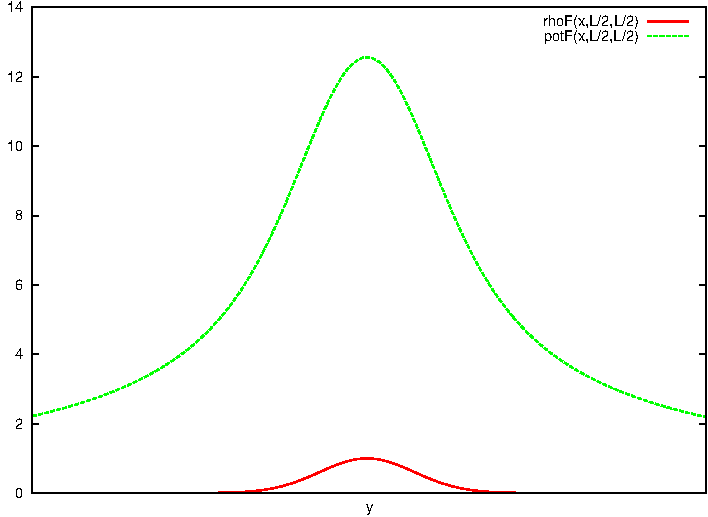
\includegraphics[width=0.8\textwidth]{rhoFpotF.pdf}
\caption{Analytic functions chosen for the Free BC Poisson Solver test}\label{fig1}
\end{figure}

\subsection*{Surfaces BC}
For Surfaces boundary conditions, we will consider an analytical density of the following type:
\be
\texttt{rhoS}(x,y,z)= f''(x) g(y) f(z) + f(x) g''(y) f(z) + f(x) g(y) f''(z)\;,
\ee
such as the potential can be written as:
\be
\texttt{potS}(x,y,z)=-4 \pi f(x) g(y) f(z)\;.
\ee
To ensure BC of surfaces type, isolated in the $y$ direction, the function $f$ must be periodic, while the function $g$ should go to zero near the borders of the simulation region.
The functions we choose are
\begin{align}
 f(x)&=e^{\cos \left(2 \pi (x-L/2)/L\right)} \\
 g(x)&=e^{-50 \frac{(x-L/2)^2}{L^2}} e^{-\left(\tan \left(\pi \frac{(x-L/2)}{L}\right)\right)^2}
\end{align}
See the figures \ref{fig2} and \ref{fig3} for a representation of these functions and for $\texttt{rhoS}(L/2,y,L/2)$ and $\texttt{potS}(L/2,y,L/2)$.
\begin{figure}[htbp]
 \centering 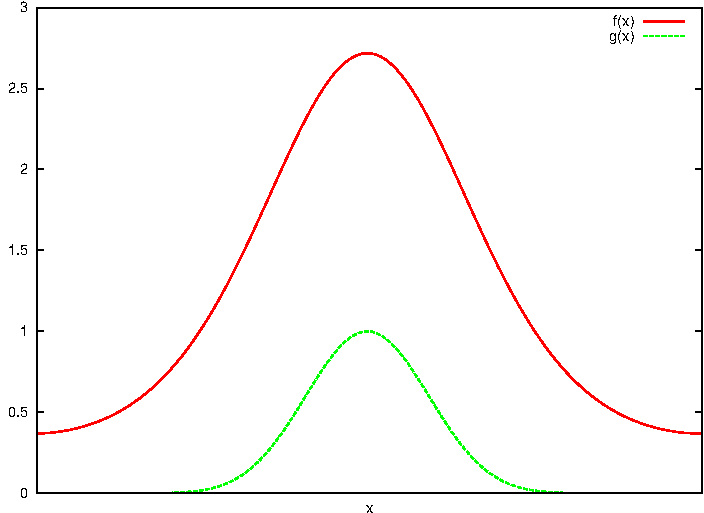
\includegraphics[width=0.6\textwidth]{fandg.pdf}
\caption{One dimensional functions chosen for constructing the analytic charge density for surfaces BC}\label{fig2}
\end{figure}
\begin{figure}[htbp]
 \centering 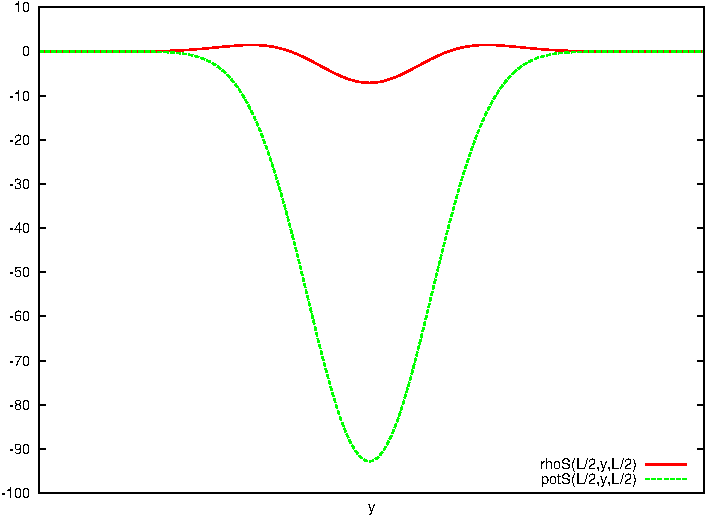
\includegraphics[width=0.6\textwidth]{rhoSpotS.pdf}
\caption{Analytic functions chosen for the Surfaces BC Poisson Solver test}\label{fig3}
\end{figure}
The density and the potential are periodic in $x$ and $z$ and go to zero (with all the derivatives) for $y$ on the border of the simulation region. This means that for this particular case such function is also compatible with a fully periodic poisson solver. 

\clearpage
\section*{Part1: Numerical accuracy of the Solver}
\begin{exercise}
For the Free BC Solver, look at the plot of the output functionsot and inspect the values of the accuracy for some choices of the grid spacings (e.g. 0.1,0.2,0.3,$\cdots$)
\end{exercise}
\begin{exercise}
Change the value of the interpolating scaling function to perform the calculation and see how the accuracy varies.
\end{exercise}
\begin{exercise}
Do the same thing for the Surfaces BC Solver.
\end{exercise}
\begin{exercise}
Suppose we need to calculate the integral
\be
\int \dd \mathbf{r} \dd \mathbf{r}' \frac{e^{-\frac{r^2}{2 \sigma^2}} e^{-\frac{r'^2}{2 \sigma^2}} }{|\mathbf{r} - \mathbf{r}'|}\;.
\ee
Can we use this program to calculate this? Which solver you should use? See how the answer varies by changing the grid spacing and the degree of Interpolating Scaling Functions.	
\end{exercise}
\begin{exercise}
We saw the the function \texttt{rhoS} is also suitable for a fully periodic treatment. The periodic Poisson Solver is able to fix the offset of the potential by fixing the zeroth Fourier component variable in the input parameters.
Which value of the \texttt{zerofc} variable must be given for obtaining the same solution of the Surface solver? Inspect the accuracy and plot the functions for some values of hgrid.
\end{exercise}
\begin{exercise}
Is it possible to do the same for the functions \texttt{rhoF}? Compare the results and plot the functions.
\end{exercise}
\clearpage
\subsection*{Part 1: Answers and discussion}
\begin{description}
 \item[Exercises 1-2-3] The accuracy values you find should be placed on curves of that kind:
\begin{center}
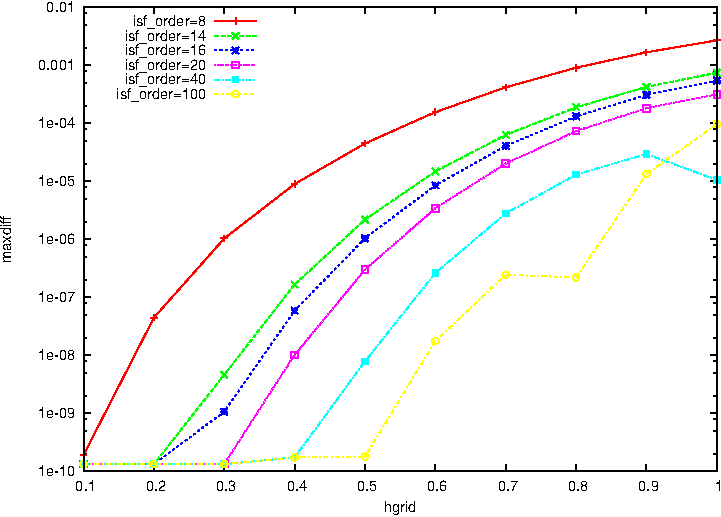
\includegraphics{accF.pdf}
\end{center}
for Free BC, while for surfaces BC we have
\begin{center}
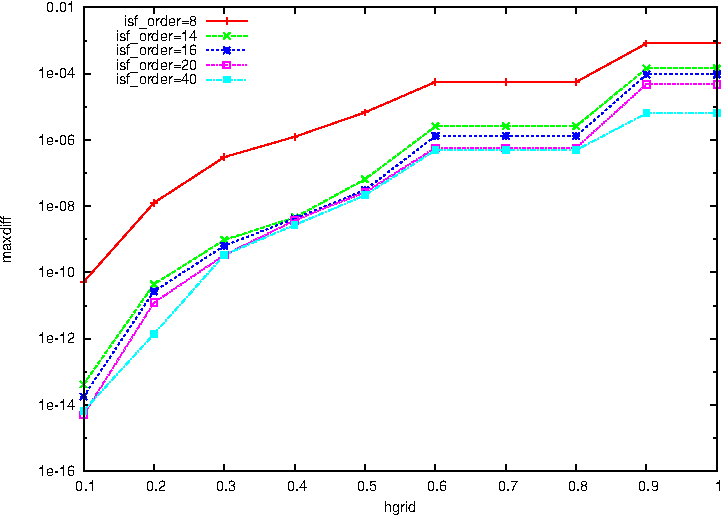
\includegraphics{accS.pdf}
\end{center}
as you can see, in the Free BC case the curves saturates at a given moment. This happens since we are using an approximation for describing the Green's function in terms of a tensor product decomposition, and this approximation has an accuracy of the order of $10^{-10}$ on a grid of about 10 atomic units. This will not happen for the Surfaces BC case. Since in this case there were no approximation used for expressing the Green's function, the limit in the accuracy is represented by machine precision.

\item[Exercise 4] The function in the integral can be seen as 
\be
\int  \dd x\,\dd y\,\dd z\,  \texttt{potF}(x,y,z) \texttt{rhoF}(x,y,z) = 2 \times \texttt{energy} \;.
\ee
Given that $\int \dd x \text{\rm{erf}}(x) = e^{-x^2} / \sqrt{\pi} + x \text{\rm{erf}}(x)$, the analytic result of the integral is
\be
4 \pi (2 \pi \sigma^2)^{3/2} \int_0^\infty \dd r \, r^2 e^{-\frac{r^2}{2 \sigma^2}}  \frac{\rm{erf}\left(\frac{r}{\sqrt{2} \sigma} \right)}{r} = 8 \left(\pi \sigma^2\right)^{5/2} = 139.94734662099890277\;,
\ee
the accuracy of the numerical results of the integral can be seen in the following plot
\begin{center}
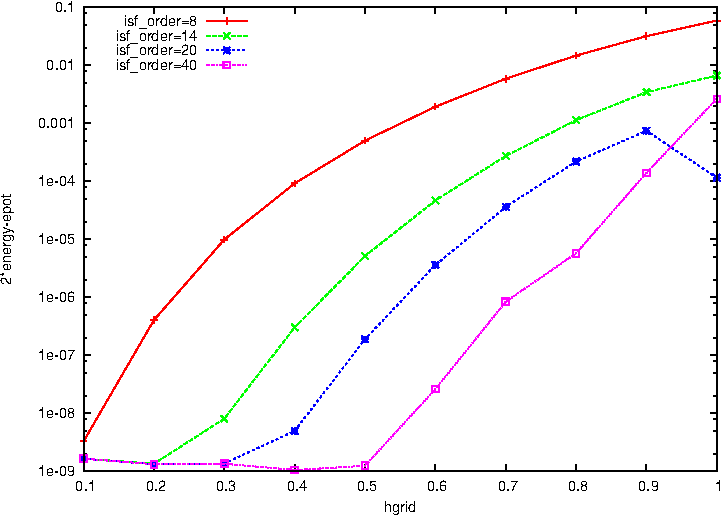
\includegraphics{emepot.pdf}
\end{center}
\newpage
\item[Exercise 5] We saw that \texttt{zerofc} represents the value of
\be
\int \dd \mathbf{r}  V(\mathbf{r}) = \text{\texttt{zerofc}}\;.
\ee
For this reason, the correct value of the variable that must be inserted in the code is
\begin{verbatim}
 zerofc=intpotS
\end{verbatim}
In such a way the result will have the same behaviour of the Poisson Solver for Surfaces BC
\begin{center}
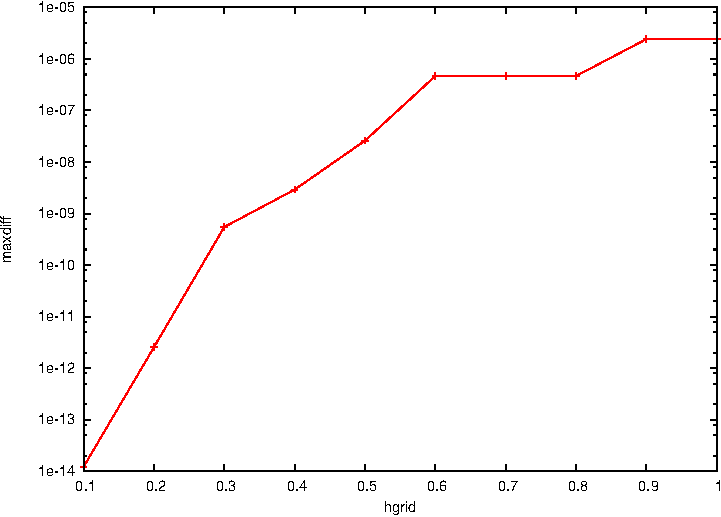
\includegraphics[width=.5\textwidth]{accP.pdf}
\end{center}
For a non-analytical case, this would require the knowledge of the ``true'' value of \texttt{zerofc} before starting the calculation, which is not possible in the great majority of tha cases.

\item[Exercise 6] The function \texttt{rhoF} cannot be passed to the periodic Poisson solver, either by fixing \texttt{zerofc = intpotF}, since the shape of the solution is not such to be treated with a periodic BC:
\begin{center}
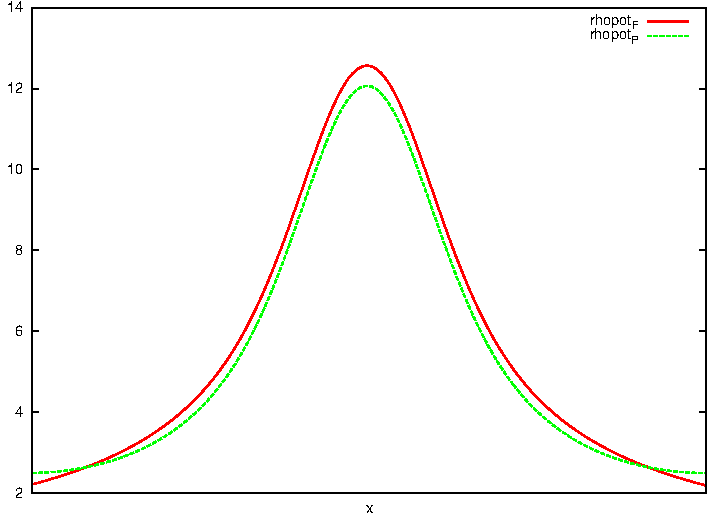
\includegraphics{PvsF.pdf}
\end{center}
Only by enlarging the simulation box we would have a solution which is closer to the analytic result. However, with a periodic solver we will \emph{never} be able to reproduce isolated BC exactly, since the Green's function for isolated BC is long-ranged.
\end{description}


\section*{Part 2: The Poisson Solver for simulating charged systems}
As pointed out before, a common fully periodic Poisson Solver is not able to determine the value of the offset of the potential. 
Consequently, some integrated quantities such as energies can be affected by this choice.
This may results in problems when performing energy differences between systems with different charges, since this will corresponds to a charge density (hence a potential) differently normalised.
The objective of this exercise is to show that this problem do not exists with our approaches, which implicitly provide the good offsets for comparing the results. In other terms, this Poisson solver can be used without problems for performing electronic structure calculations with charged systems on isolated or surface type BC.

\begin{exercise}
Calculate the potential energy \texttt{epot} for the potentials coming from the previous exercise with the Isolated and Surfaces BC for a value of the grid spacing at your choice, with a reasonable accuracy.
Calculate both the results with the Periodic Poisson solver. Which value of \texttt{zerofc} must be given to the Poisson solver for having the same energy?
\end{exercise}
Now let us imagine to change the total charge of the system, by multiplying by a factor (say two) the charge density. For linearity, the potential V coming out from the Poisson equation is multiplied by two. The same will happen for the value of \texttt{epot}.
\begin{exercise}
Do the same calculations of the previous exercise with a charge density multiplied by two and perform the energy differences with the ``single charge'' results. Does the results obtained with the periodic solver are the same? Should we change the value of \texttt{zerofc}  to get the same results? If yes, how?
\end{exercise}
\subsection*{Part 2: Answers and discussion}
\begin{description}
 \item[Exercise 7] Knowing that the trial wavefunction psi is normalised, by shifting the potential $V'=V+c$, we also have $\texttt{epot}'=\texttt{epot}+ c \times \texttt{n1*n2*n3*hgrid**3}$
Hence, for Isolated BC the correct value of \texttt{zerofc} is
\begin{multline}
 \texttt{zerofc}=\Bigl[\texttt{epot}_F - \texttt{epot}_P(\texttt{offset=0})\Bigr]\times\texttt{n1*n2*n3*hgrid**3} =\\= 3.053506154731705  \texttt{*n1*n2*n3*hgrid**3}
\end{multline}
to give an \texttt{epot} of 10.260398641217504.

For surfaces BC the correct value of \texttt{zerofc} is again \texttt{intpotS}, since for this value the solutions are identical. The value of \texttt{epot} is -74.77033746378227

\item[Exercise 8] 
The linearity in the value of \texttt{epot} which is guaranteed by a full Green's function treatment cannot be achieved with a periodic Poisson solver. Indeed, for an isolated system the only way to double the energy of the system when the density double is to double also the offset of the potential. Moreover, the value of the energy difference wil be explicitly dependent on the initial offset, which makes all the results meaningless. The Green function treatment choices automatically the \emph{only} offset which is compatible with the choice of the BC, making thus the treatment of charged systems easy and immediate.

\end{description}
\clearpage
\section*{Theory: Poisson Solver with different boundary conditions}
\textit{Note: this appendix will explain in some words the basical theory behind this Poisson Solver. You can skip directly to the exercises and use this section only in case of need.}\\
A Poisson solver is a computer program which solves the Poisson equation
\be\label{PSeq}
\nabla^2 V(x,y,z) = - 4 \pi \rho(x,y,z)\;.
\ee
In other terms, given a function (``density'') $\rho(x,y,z)$ defined on a three-dimensional domain $\Omega$, the Poisson Solver will output another function $V(x,y,z)$ (``potential''), defined on the same domain, which satisfy eq. \eqref{PSeq}.

Of course, for a given density $\rho$ there are infinite solutions to the Poisson equations: indeed, for $V$ which satisfy $\eqref{PSeq}$, also $V'=V+H$, with $\nabla^2 H=0$ is a possible solution. Among the possible solutions, the one which fits best in the problem under consideration depends on the boundary conditions (BC) of the domain.

\subsection*{Isolated BC}
For an infinite domain ($\mathbb R^3$) with isolated BC, the solution can be found via the Green's function $G(r)$:
\begin{align} 
G(r)=\frac{1}{r}\;;&\qquad\nabla^2 G(\sqrt{x^2+y^2+z^2}) = -4 \pi \delta(x) \delta(y) \delta(z) \label{isolatedGF} \\
&\Downarrow \notag \\
V(x,y,z)&=\int \dd x' \dd y' \dd z'\frac{\rho(x',y',z')}{\sqrt{(x-x')^2+(y-y')^2+(z-z')^2}}\;.\label{solutionIBC}
\end{align}
For a density which satisfy isolated BC, a potential defined in this way automatically goes to zero at infinity.

\subsection*{Surfaces BC}
Another example can be provided with surfaces BC, namely for domains which are isolated in one direction (say $y$) and periodic in $x$ and $z$, with periods $L_x$ and $L_z$ respectively. A function $f$ which lives in such a domain can be expanded as
\be \label{expansionSBC}
f(x,y,z)=\sum_{p_x,p_z} e^{-2\pi i\left(\frac{p_x}{L_x} x + \frac{p_z}{L_z} z\right)}
f_{p_x,p_z}(y)\;,
\ee
without any loss of generality.
For such functions the Poisson equation become
\be
\left(\partial_y^2 - \mu_{p_x,p_z}^2 \right) V_{p_x,p_z}(y) = \rho_{p_x,p_z}(y)\;,
\ee
where $\mu_{p_x,p_z}^2=4 \pi^2 (p_x/L_x)^2 +(p_z/L_z)^2$.
With the use of the Green's function of the one-dimensional Helmoltz equation \emph{for isolated BC}
\begin{align}
\left(\partial_y^2 - \mu^2 \right) G(\mu; y) &= \delta(y) \label{surfacesGF}\;; \\
G(\mu;y)=
\begin{cases}
 -\frac{1}{2 \mu} e^{-\mu |y|} & \mu > 0 \\
\frac{1}{2}|y| & \mu=0
\end{cases}\;,
\end{align}
the components of the potential can be carried out:
\begin{equation}
 V_{p_x,p_z}(y) = \int \dd y' G(\mu_{p_x p_z}; y-y') \rho_{p_x,p_z}(y')\;.
\end{equation}
By construction, the potential defined in this way will satisfy surfaces BC.

\subsection*{Periodic BC}
The last example that can be shown is probably the most commonly referenced, namely fully periodic BC with periods $L_x$, $L_y$ and $L_z$.
In that case the Poisson equation \eqref{PSeq} become simply an algebraic equation between the Fourier components of $V$ and $\rho$:
\be
V_{p_x,p_y,p_z} = \frac{1}{\pi}\frac{1}{\left(\frac{p_x}{L_x}\right)^2 + \left(\frac{p_y}{L_y}\right)^2 +\left(\frac{p_z}{L_z}\right)^2} \rho_{p_x,p_y,p_z}\;,
\ee
where $\rho$ and $V$ are developed following the expansion
\be
f(x,y,z)=\sum_{p_x,p_y,p_z} e^{-2\pi i\left(\frac{p_x}{L_x} x +\frac{p_y}{L_y} y+ \frac{p_z}{L_z} z\right)}
f_{p_x,p_y,p_z}\;.
\ee
For this choice of the BC the zero-th fourier component of the potential $V_{0,0,0}=\int_{\Omega} V$
cannot be determined by the Poisson equation. In other terms, the periodic BC are compatible with any choice of the offset: for any valid $V$, also $V'=V+c$, where $c$ is a constant function, is a valid analytic solution of eq. \eqref{PSeq}.
The calculation of the quantity (``Hartree energy'')
\be \label{ehart}
E_H=\frac{1}{2}\int_\Omega \dd x\, \dd y\, \dd z\, V(x,y,z) \rho(x,y,z)
\ee
will depend explicitly on the choice of the offset.

\end{document}


